%
% File: Calibration.tex
% Author: Ran Itay
% Description: EFT analysis
%
\let\textcircled=\pgftextcircled

\chapter{Calibration System for Xenon1T} \label{chap:calib}

\initial{O}ne of the most important prerequisite for having a successful detector is a good understanding of the response for different types of interactions. In "low-background" experiments the usual technique for quantifying the detector response for different radiation types, is by creating a controlled data sample for each type of interaction. This sample is obtained by exposing the detector to a radioactive source with intensity which is order of magnitude greater than the background rate. This insures that the events in the detector are coming from a specific type of interaction, with a well defined energy. The study of these induced signals is known as "\textit{detector calibration}" 

The two measurable of XENON100 and XENON1T are the prompt scintillation (S1) and the proportional scintillation (S2). The efficiency of of detecting the scintillation light determines the energy threshold of the detector. Both light and charge yields can be attenuated by impurities in the LXe. 

The non uniformity of scintillation light collection signal s due to solid angle effects, Rayleigh scattering length, reflectivity, transmission of the electrodes, etc. lead to a
position-dependent S1 signal. Extracted electrons are absorbed by impurities, mainly by oxygen and water, the number of electrons reaching the GXe is depth (z) dependent. Hence a correction to the energy scale both in S1 and S2 should be applied. This calibration is known as light and charge collection. 

Most of the background of XENON1T is due to electromagnetic interactions, predominantly, $\gamma$s, interacting in the target. Most of the background events occur near the TPC walls, this is due to the stopping power of LXe. Therefore, most of the background rejection is achieved through fiducialization, namely limiting the science data to a smaller FV volume. In addition to that the ratio between S2 and S1 for NRs (expected signal) and ERs (background) is different in nature. The main discrimination power of XENON1T is via this ratio. A good understanding of the different response to the two interaction types is important to quantify the background leakage distribution. Also the response for NR is important to produce data-MC matching. This is, amongst other, important to understand the acceptance of the different data selection criteria applied in the analysis process. This calibration is known as "NR and ER bands"    

The trivial and easiest approach to calibrate the detector is the one applied in XENON100. Simply place a gamma source outside the detector and create the controlled data sample. However, this approach is not applicable for XENON1T due to various reasons. The main obstacle is to deploy the source inside the water tank. Moreover, for each calibration type, events need to fulfill cretin data selection criteria which dictates the rate and energies needed. 

For the light and charge collection calibration the full absorption peak is used; therefore even low-energetic sources, such as \Cs\ (662 keV $\gamma$s) can be used to produce a fairly large data sample in a reasonable time. For the ER band calibration, just placing a source near the detector is not sufficient. There are more  data selection criteria needed for this calibration. 

A good ER band calibration event should have low energy deposition ($2-15\keVee$), should scatter only once in the detector, should occur inside the FV an should scatter only once in the detector. Notice that the diameter of XENON1T TPC is $\sim 1$\,meter meaning a $\gamma$ needs to penetrate the FV (travel $\sim 10$\,cm inside LXe) scatter in a small angel and travel outside of the TPC($\sim 90$\,cm) without scattering again in order to produce a good calibration event. The probability for that to happen, even for a 2\,MeV source is very low $\sim 10^{-7}$. Because the detector cannot process data at high rates, the amount of time needed for this calibration is extremely long, and a new approach is needed.

Internal calibration techniques, in which a short lived radioactive source is dissolved inside the LXe is one of the calibration methods used in XENON1T. The radioactive sources used are: $^{83m}\mathrm{Kr}$, tritated methane $\mathrm{CH_3T}$ and $^{220}\mathrm{Rn}$.    




%Using an external source in order to calibrate XENON1T, imposes some difficulties. Due to the Xenon self shielding, it is unlikely for a gamma to penetrate at least 10cm of xenon scatter in a small angle (low energy deposition) and travel ~90 cm outside the cryostat. The rate of events in the cryostat is limited from several aspects such as, “pile ups”, PMT bases, and “dead time” after large S2s. The idea of going into “pile-up mode” is unlikely to work due to the PMT base design. Therefore, re- examination of calibration techniques was needed. In this section I will present the calibration rates for the new selected technique which is now in manufacturing stages and will be installed in XENON1T in the near future.

In this section I describe the new technique for external calibration, mainly ER band calibration, including the radioactive sources used, the holders of the sources which will confine there radiation to a smaller solid angle, and the system which drives the sources into place. The detector has been modeled in details using the GEANT4 toolkit~\cite{AGOSTINELLI2003250} which provides also the nuclear and electronic recoil differential cross-section. Using this powerful toolkit one simulates the response of the detector to the different sources and study the expected response of the detector. 



\section{Radioactive source}
\label{sec:source}
\subsection{ER band calibration}
Since The mean free path of $\gamma$ traveling in xenon is of the order of several cm (8.3\,cm for a 1\,MeV $\gamma$), depending on the $\gamma$'s energy~\ref{fig:MFP}, a good $\gamma$ calibration source should emit energetic enough $\gamma$s to penetrate to the FV. 

\begin{figure}
	\begin{center}
	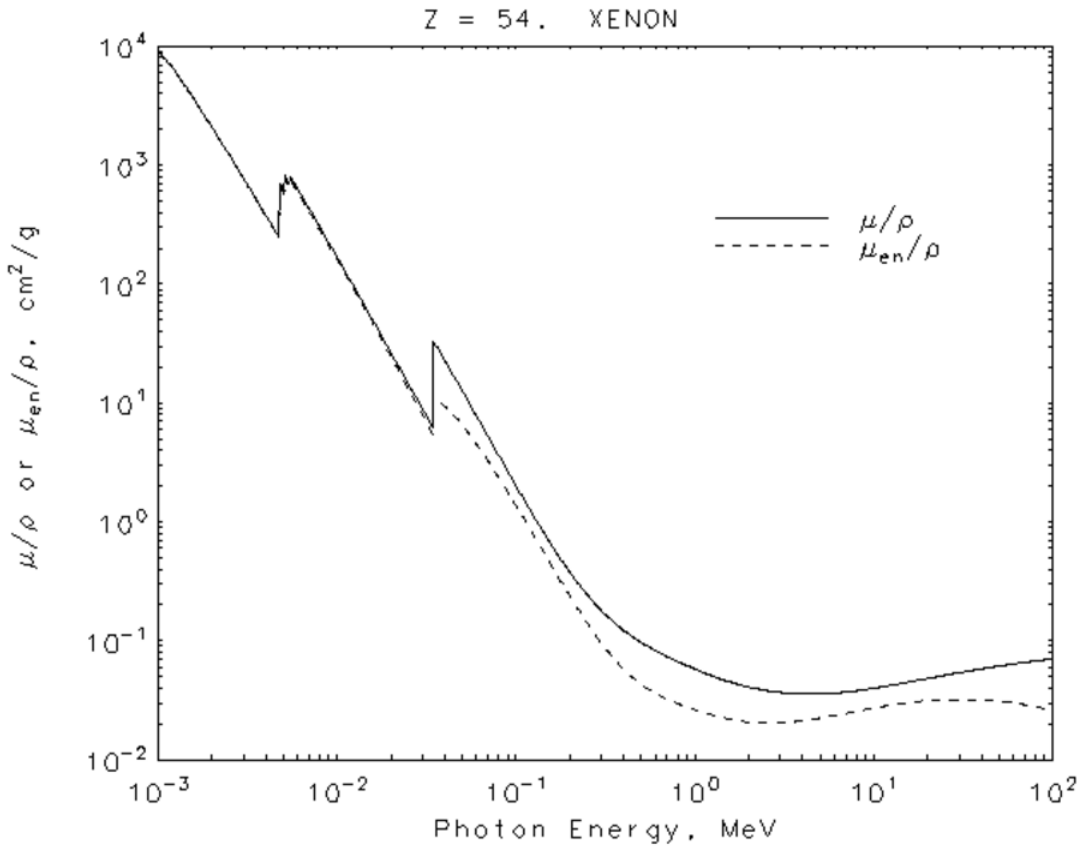
\includegraphics[width=\textwidth]{figs/NISTAttXenon.png}%  
		\caption{\label{fig:MFP} Attenuation coefficient of Xe. The relevant density for LXe is 3\,g/cc.}
		\end{center}
	
\end{figure} 

After careful examination a \Th\ source is selected, see decay chain is in Fig.~\ref{fig:th228} The source is encapsulated in SS and with an M4 thread. All $\beta$ and $\alpha$ decays will not reach the xenon because the source is encapsulated, leaving only $\gamma$ radiation. The $\gamma$ emission line for ER band calibration is the one coming from $^{208}\mathrm{Tl}$ with energy of 2614\,keV and intensity of 99~\%. Less energetic $\gamma$ emission lines will penetrate the SV and trigger the PMTs but will not proceed to the FV and hence will be treated as background. 

\begin{figure}
	\begin{center}
	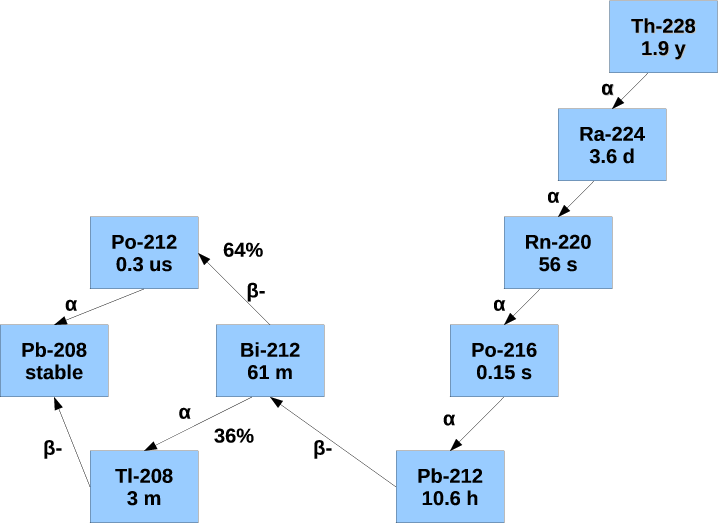
\includegraphics[height= 0.5\textheight]{figs/Th228Check.PNG}% Here is how to import 
		\caption{\label{fig:th228} \Th\ decay chain }
		\end{center}
	
	\end{figure} 
 
In order to estimate the percentage of good calibration events from total triggering all spectral lines are simulated, however only the 2614 keV events are considered as signal events, while the rest are treated as background.  
A summarize of the more energetic $\gamma$ lines from \Th\ decay chain is presented in Table~\ref{table:isotope}.
\begin{table}
\begin{center}
\resizebox{\textwidth}{!}{
 \begin{tabular}{||c c c c||} 
 \hline
 Energy (keV) & SV prob(\%) & Isotope & Intensity(\%) \\ [0.5ex] 
 \hline
 511 & 0.27 & $^{208}\mathrm{Tl}$ & 22.8 \\ 
 \hline
 583 & 0.35 & $^{208}\mathrm{Tl}$ & 85 \\
 \hline
 727 & 0.51 & $^{212}\mathrm{Bi}$ & 6.7 \\
 \hline
 763 & 0.54 & $^{208}\mathrm{Tl}$ & 1.8 \\
 \hline
 861 & 0.64 & $^{208}\mathrm{Tl}$ & 12.4 \\  
 \hline
 1621 & 1.15 & $^{212}\mathrm{Bi}$ & 1.5 \\  
 \hline
 2614 & 1.5 & $^{208}\mathrm{Tl}$ & 99 \\ [1ex] 
 \hline
\end{tabular}
}
\caption{High energy gamma lines from \Th\ decay chain}
\label{table:isotope}
\end{center}
\end{table}

All decays from $^{208}\mathrm{Tl}$ have an attenuation factor of 36\% which is the branching ratio of $^{212}\mathrm{Bi} \rightarrow ^{208}\mathrm{Tl}$
In total the percentage of 2614\,keV events in the SV is 0.69\% of total source activity.

\subsection{Charge collection efficiency}
The calibration of the charge collection efficiency is done with less restrict data selection criteria than the ER band calibration. A good calibration sample for this calibration should have a well defined characteristic feature obtained from the source in various z-positions. By comparing the feature dependency on height a charge collection efficiency map is produced. An easy and well defined feature is the full absorption peak. 

\Cs\ source which emits a 662\,keV $gamma$, is selected for this calibration. The decay of \Cs\ is shown in Fig~\ref{fig:Cs}. The source is deposited inside a 25\,mm diameter disk. 


\begin{figure}
	\begin{center}
	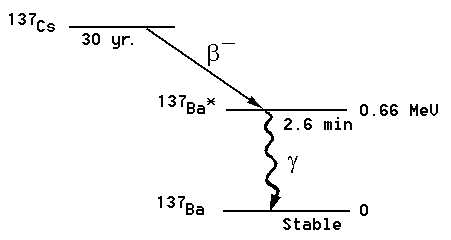
\includegraphics[width=0.55\textwidth, height= 0.3\textheight]{figs/Cs137.png}% Here is how to import 
		\caption{\label{fig:Cs} \Cs\ decay}
		\end{center}
	
	\end{figure} 

\section{Collimators} \label{sec:Col}
 
Large portion of the $\gamma$s arriving to the SV are scattered at the outskirts of the SV and don't reach the FV, these events trigger the PMTs however are of no use for ER band calibration. In order to lower this portion the gamma source will be placed behind a frame, with a conical hole, such that the solid angle of the hole will cover just the FV when the source is located at the center of the TPC (see Fig. ~\ref{fig:Colimator}). 
%
%\begin{figure}[t!]
%\centering
%\begin{minipage}{3.3cm}
%    \centering
%    \subtop[]{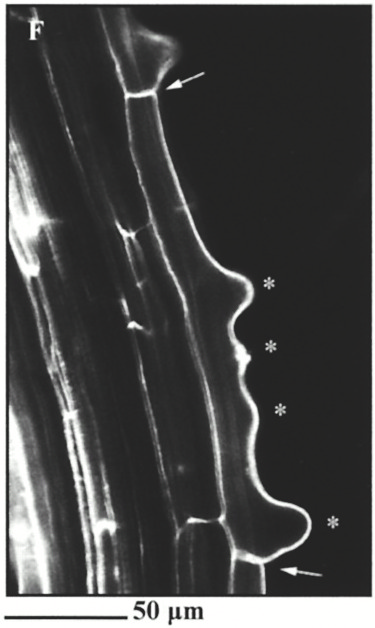
\includegraphics[height=0.28\textheight]{fig01/Nswellings}\label{sf:multiRH02a}}
%\end{minipage}
%\hspace{0.5cm}
%\begin{minipage}{3.3cm}
%    \centering
%    \subtop[]{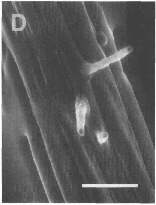
\includegraphics[height=0.27\textheight]{fig01/Mswellings}\label{sf:multiRH02b}}
%\end{minipage}
%\hspace{1.3cm}
%\begin{minipage}{3.3cm}
%    \centering
%    \subtop[]{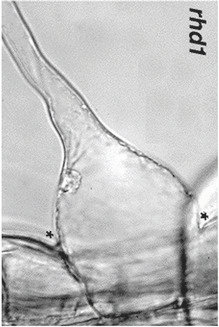
\includegraphics[height=0.27\textheight]{fig01/rhd1}\label{sf:multiRH02c}}
%\end{minipage}

 \begin{figure}
   \centering
    \begin{minipage}[c]{0.49\textwidth}
    \centering
    \subbottom[]{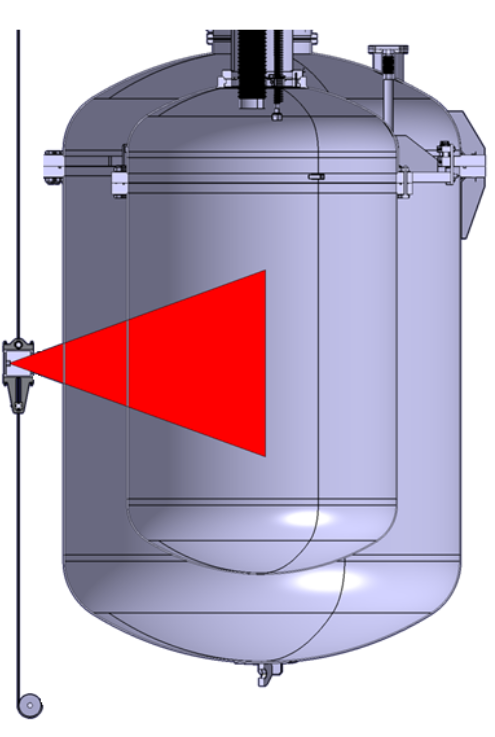
\includegraphics[width=\textwidth]{figs/collimator2.png}
%        \caption{The cryostat and the collimator shining just some of the FV }
        \label{subfig:colimator_cryo}}
    \end{minipage}
    \begin{minipage}[c]{0.4\textwidth}
	\centering    
        \subbottom[]{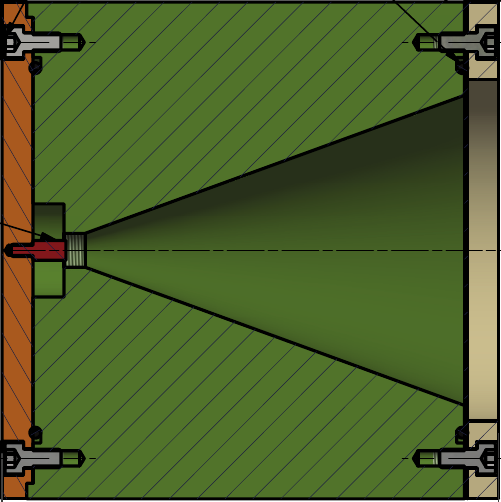
\includegraphics[width=\textwidth]{figs/CollimatorCAD.png}
%        \caption{a CAD design of the collimator with the conical hole.}
        \label{subfig:colimator_Cart}}
    \end{minipage} 
    \caption{ (a) The cryostat and the collimator shining just some of the FV (b) a CAD design of the collimator with the conical hole. \label{fig:Colimator}}
\end{figure}

There are two types of collimators: a 16X16X16\,cm collimator which will just move vertically on a belt (I-Collimator), and a 10X10X10\,cm collimator which passes below the cryostat (U-Collimator). 
Both collimators are made of Tungsten with a $45\deg$ aperture, sealed with a 1\,mm SS plate to reduce the amount of water an emitted $\gamma$ travels through. 
The two collimators are designed to host both threaded sources (\Th) and disk sources (\Cs). An M12 thread is located in front of the  
source position to allow adding an attenuator.
 
The collimators are attached to belts that drives them to various calibration positions. The larger collimator is attached to an I-belt and moves only vertically, see Fig~\ref{fig:IUBeltpic}. The smaller collimator is attached to a U-belt, that passes below the cryostat, see Fig~\ref{fig:IUBeltpic}. The two I belts are connected to ports 5 and 11 while the U belt is connected to ports 12 and 7,on the water tank's top flange see Fig.~\ref{fig:topFlange} 


\begin{figure}
	\begin{center}
	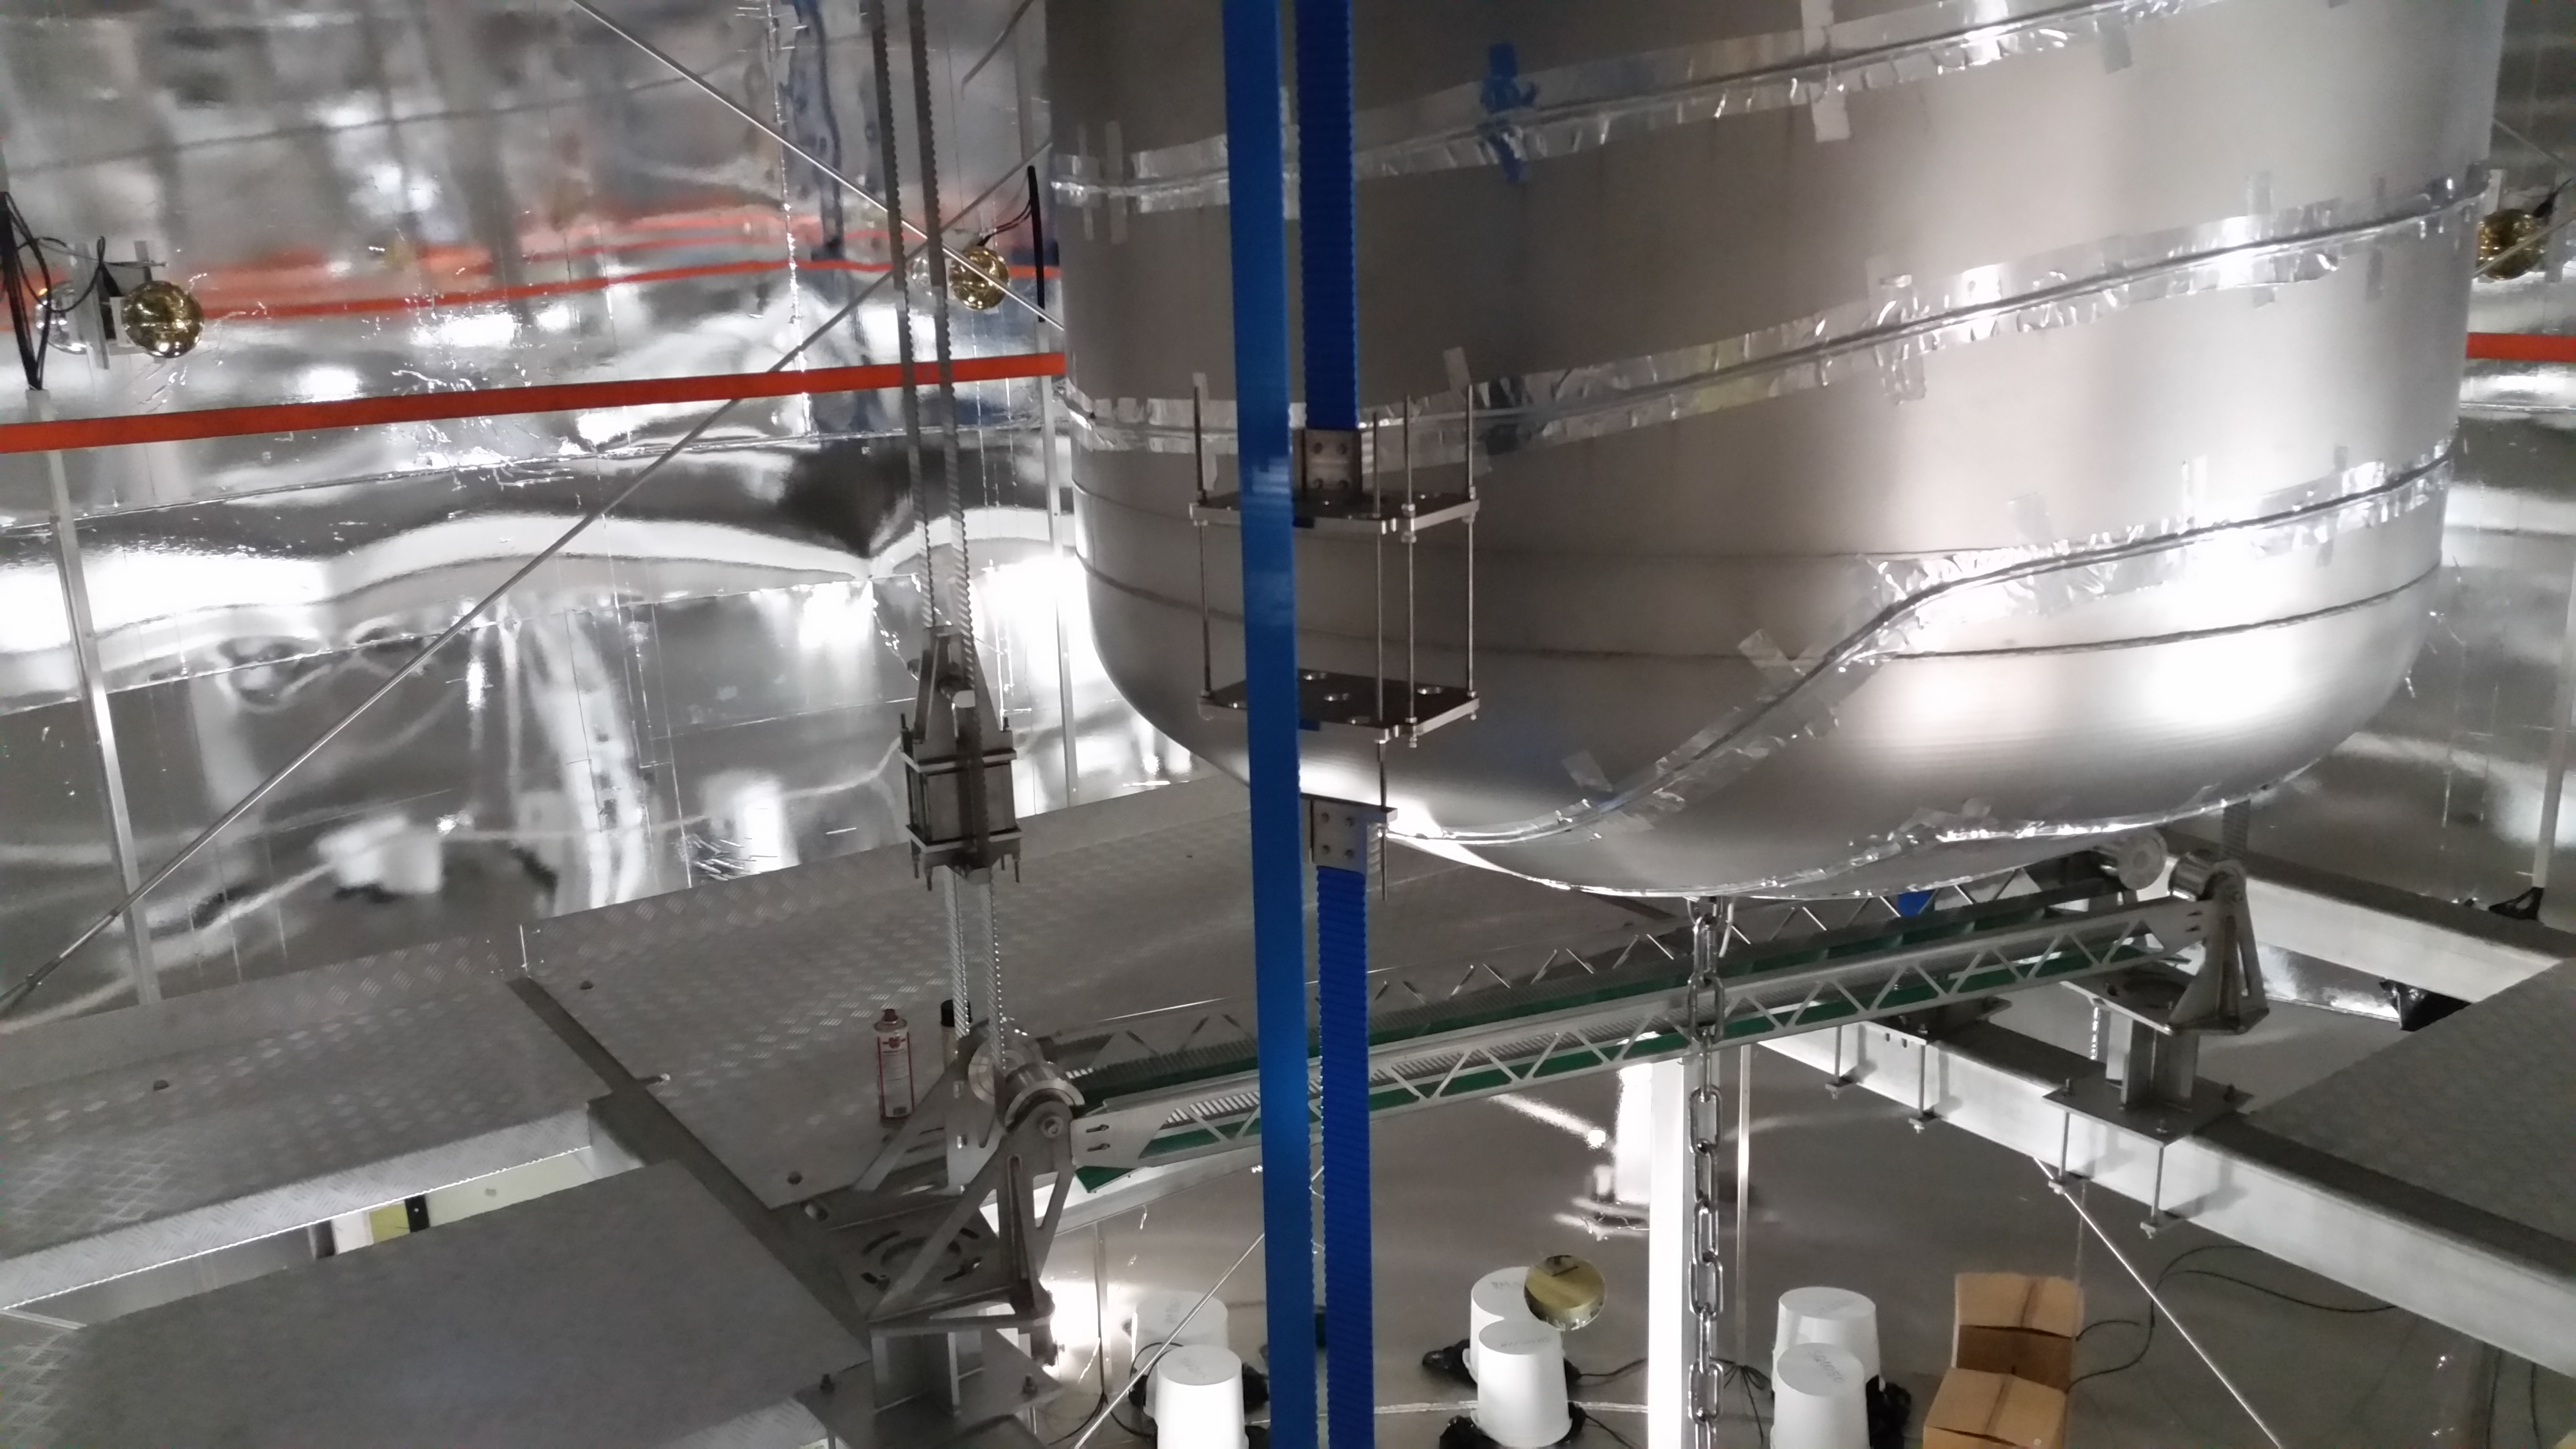
\includegraphics[width=\textwidth]{figs/IUBeltPic.jpg}% Here is how to import 
		\caption{\label{fig:IUBeltpic}A picture of the two belts. The blue belt is the I-Belt (currently not the I-Belt in use). The grey belt is the U-Belt (with the U-Collimator mounted), which passes below the cryostat.}
		\end{center}
\end{figure}



\begin{figure}
	\begin{center}
	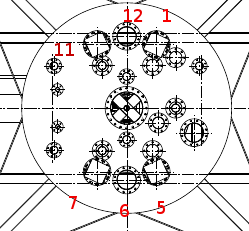
\includegraphics[width=0.55\textwidth]{figs/waterTankTopView.png}% Here is how to import 
		\caption{\label{fig:topFlange} A top view of the water tank }
		\end{center}
	
	\end{figure}
\subsection{Simulation} \label{subsec:simulation}

In order to decide the source activity and collimator dimensions, a MC simulation using the GEANT4 toolkit is used. The DAQ rate assumed for this study is 350\,Hz. The response of the detector to 2614\,keV$\gamma$'s is simulated. Other $\gamma$'s coming from the detector are assumed to be background, and are considered only for rate calculations.

The results from the simulation of the I-Collimator which points to the center of the detector are shown in table~\ref{table:ICol}, in Fig~\ref{fig:IBelt} are the original momentum-direction of $\gamma$s which do not produce a "good" calibration event. This is of importance to verify only events coming from the collimator opening will reach the detector's SV.


\begin{table}
\begin{center}
\resizebox{0.8\textwidth}{!}{
 \begin{tabular}{||c c||} 
 \hline
 number of simulated events & 2e9 \\ 
 \hline
 number of recorded events (SV) & 2.5e7 \\
 \hline
 number of good events & 53 \\
 \hline
 good evts/day @ 350Hz  & $65 \pm 8$ \\
 \hline
 evt/day after bkg reduction & 45 \\  
 \hline
\end{tabular}
}

\caption{result of GEANT4 simulations for a 16X16X16cm collimator with an aperture of $45 \deg$, a good event is an event that scattered only once in the FV with energy deposition of 2-15 keVee}
\label{table:ICol}
\end{center}
\end{table}


\begin{figure}
   \centering
    \begin{minipage}[b]{0.49\textwidth}
    \subbottom[]{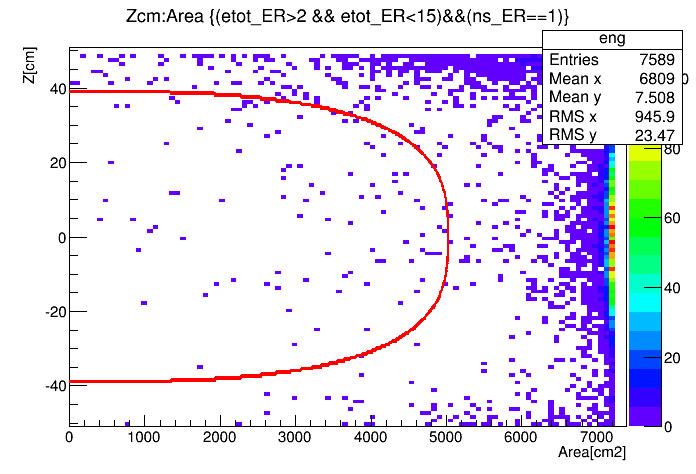
\includegraphics[width=\textwidth]{figs/scatter45deg16X16X16.png}
%        \caption{scatter of good calibration events in the SV, the red line is the border of the FV }
        \label{subfig:IBeltScatter}}
    \end{minipage}
    \begin{minipage}[b]{0.4\textwidth}
        \subbottom[]{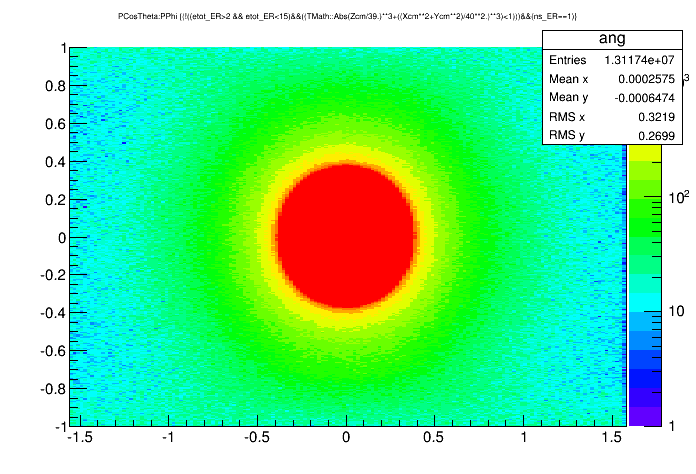
\includegraphics[width=\textwidth,height=0.23\textheight]{figs/angles16}
%        \caption{Intial momentom of background events i.e., events which trigger PMT's and do not meet all three conditions, FV, single scattered, and energy deposition range} 
        \label{subfig:IBeltAngle}}
    \end{minipage} 
    \caption{(a) scatter of good calibration events in the SV, the red line is the border of the FV  (b) Intial momentom of background events i.e., events which trigger PMT's and do not meet all three conditions, FV, single scattered, and energy deposition range \label{fig:IBelt}
}
\end{figure}



The detector is attached via a spring to the water tank's floor, this is done to apply force against the detector's buoyancy while filling water. Therefore the U-belt cannot pass underneath the center of the detector. This causes the collimator to be in a small angle with respect to the center of the detector.
The results of the simulation of the U-Collimator are shown in table~\ref{table:UCol} and Fig.~\ref{fig:UBelt}.



  

% 
%\subsection{U Collimator}
%\label{subsec:U_Belt}
%
%This 10X10X10cm collimator will be attached to one belt which will be connected to ports 11 \& 7. Due to the direction of the belt the collimator will not shine directly the center of the TPC. At the moment it will serve for ER calibration, and electron lifetime. However because it passes below the cryostat it will be used for other types of calibration. The results from GEANT4 simulation of this collimator are shown in Table~\ref{table:UCol} and Fig~\ref{fig:UBelt}  


\begin{table}
\begin{center}
\resizebox{0.8\textwidth}{!}{
 \begin{tabular}{||c c||} 
 \hline
 number of simulated events & 4e9 \\ 
 \hline
 number of recorded events (SV) & 4.05e7 \\
 \hline
 number of good events & 58 \\
 \hline
 evt/day @ 350Hz good evts & $43 \pm 6$ \\
 \hline
 evt/day after bkg reduction & 30 \\  
 \hline
 Source activity & 80kBq \\ [1ex] 
 \hline
\end{tabular}
}
\caption{result of GEANT4 simulation for a 10X10X10cm collimator with an aperture of $45 \deg$, a good event is an event that scattered only once in the FV with energy deposition of 2-15 keVee}
\label{table:UCol}
\end{center}
\end{table}


\begin{figure}
   \centering
    \begin{minipage}[c]{0.49\textwidth}
    \subbottom[]{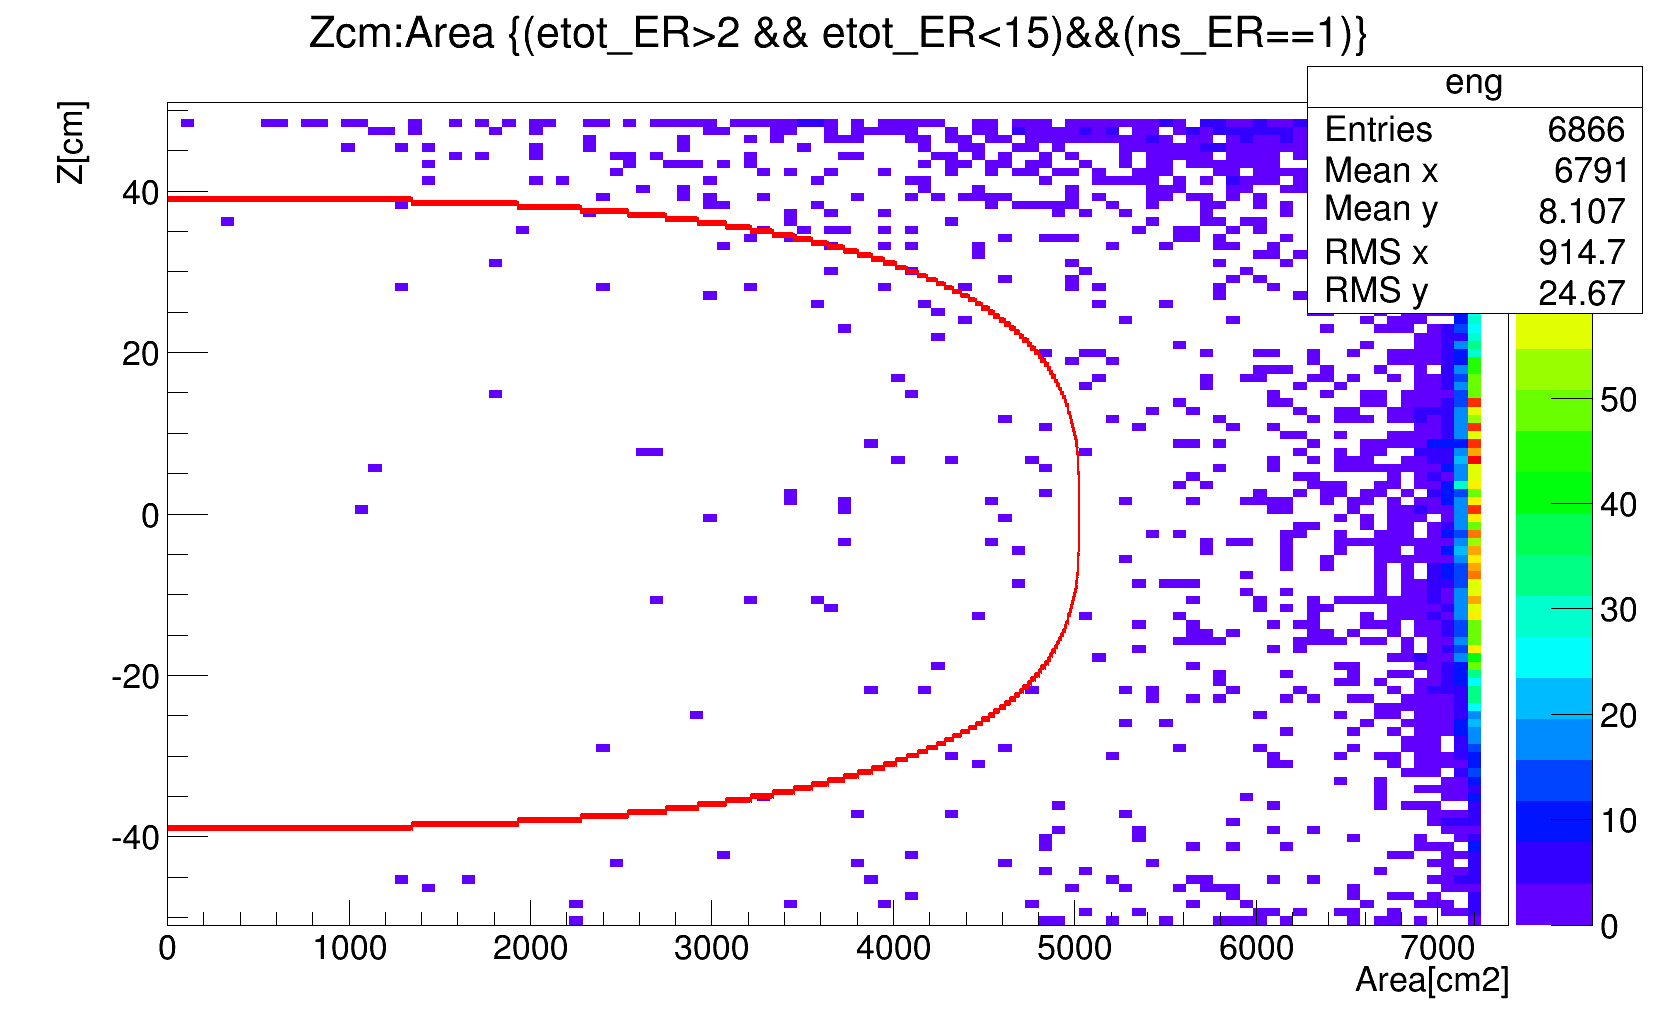
\includegraphics[width=\textwidth]{figs/ScatterPlot10X10X10NonCenteredSymetric.png}
%        \caption{scatter of good calibration events in the SV, the red line is the border of the FV }}
        \label{subfig:UBeltScatter}}
    \end{minipage}
    \begin{minipage}[c]{0.4\textwidth}
        \subbottom[]{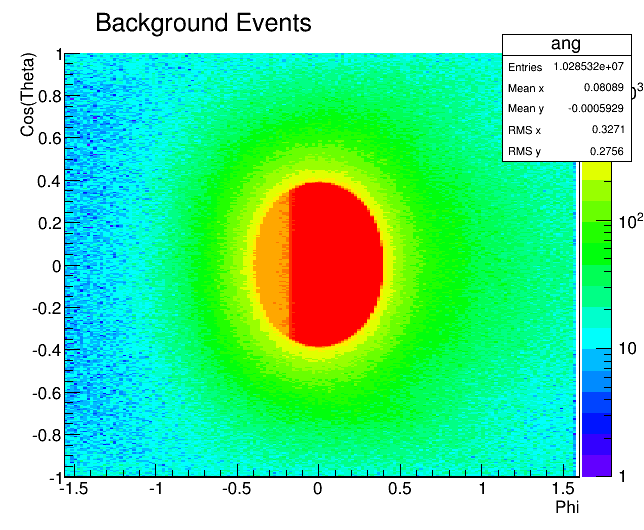
\includegraphics[width=\textwidth]{figs/Ang10X10X10NonCenteredSymetric.png}
%        \caption{Intial momentom of background events i.e., events which trigger PMT's and do not meet all three conditions, FV, single scattered, and energy deposition range} 
        \label{subfig:UBeltAngle}}
    \end{minipage} 
    \caption{(a) scatter of good calibration events in the SV, the red line is the border of the FV (b) Intial momentom of background events i.e., events which trigger PMT's and do not meet all three conditions, FV, single scattered, and energy deposition range \label{fig:UBelt}
}
\end{figure}

\subsection{First Results}
\label{subsec:FirstResults}

%TODO write this section 
